% pdflatex -shell-escape -interaction=nonstopmode main.tex && pdflatex -shell-escape -interaction=nonstopmode main.tex

\chapter{Definitionen}

% \begin{itemize}
%     \item Einführung in ML Algorithmen
%     \item ``Im folgenden werden wir ein paar Möglichkeiten in Betracht ziehen wie man Genetische Algorithmen für Black Box Optimierung benutzen kann''
%    \item ``Ausserdem verknüpfen wir diese mit einer Reduzierung vom Suchraum durch Fouriertransformationen und verwenden verschiedene Kodierung der Individuen, durch Normalverteilungen und direkt durch Zahlen''
% \end{itemize}

Dieses Kapitel bietet Einblick in die Grundlagen von \textbf{Genetischen Algorithmen} (Kap. 2.1) im Zusammenhang mit \textbf{neuronalen Netzen} (Kap 2.2.1) und der \textbf{Cross Entropy Method} (Kap. 2.5). Außerdem werden einige Verbesserungen zu den naiven Methoden besprochen, wie die Reduzierung des Suchraums durch \textbf{Fouriertransformationen} und die Einführung von einer \textbf{kooperativen Evolution} durch Hinzufügen von einer neuen Aktion zu dem Ablauf des genetischen Algorithmus.

    \section{Genetische Algorithmen}
        % ``Die Motivation von Genetischen Algorithmen kam aus der Natur bla blubb''\\
        % ``Im Folgenden behandeln wir die grundlegenden Operationen die einen GA ausmachen''

        % Ein Genetischer Algorithmus gehört zu den \textbf{unsupervised Learning} Methoden, die sich als Ziel setzen eine verborgene Struktur zu analysieren, ohne zu gekenntzeichnete Daten zu haben. John Holland

        Ein genetischer Algorithmus, im folgenden als \textbf{GA} abgekürzt, ist ein Optimierungsverfahren, das von der natürlichen Selektion und Evolution inspiriert ist. Ein formaler Leitfaden findet sich im Fundamentalwerk zu Genetischen Algorithmen \cite{ga}.\\[2mm]
        Stellen wir uns anschaulicher Weise eine Gruppe Gazellen und einen Geparden vor.\\

        \begin{figure}[htbp]
            \begin{subfigure}{0.5\textwidth}
                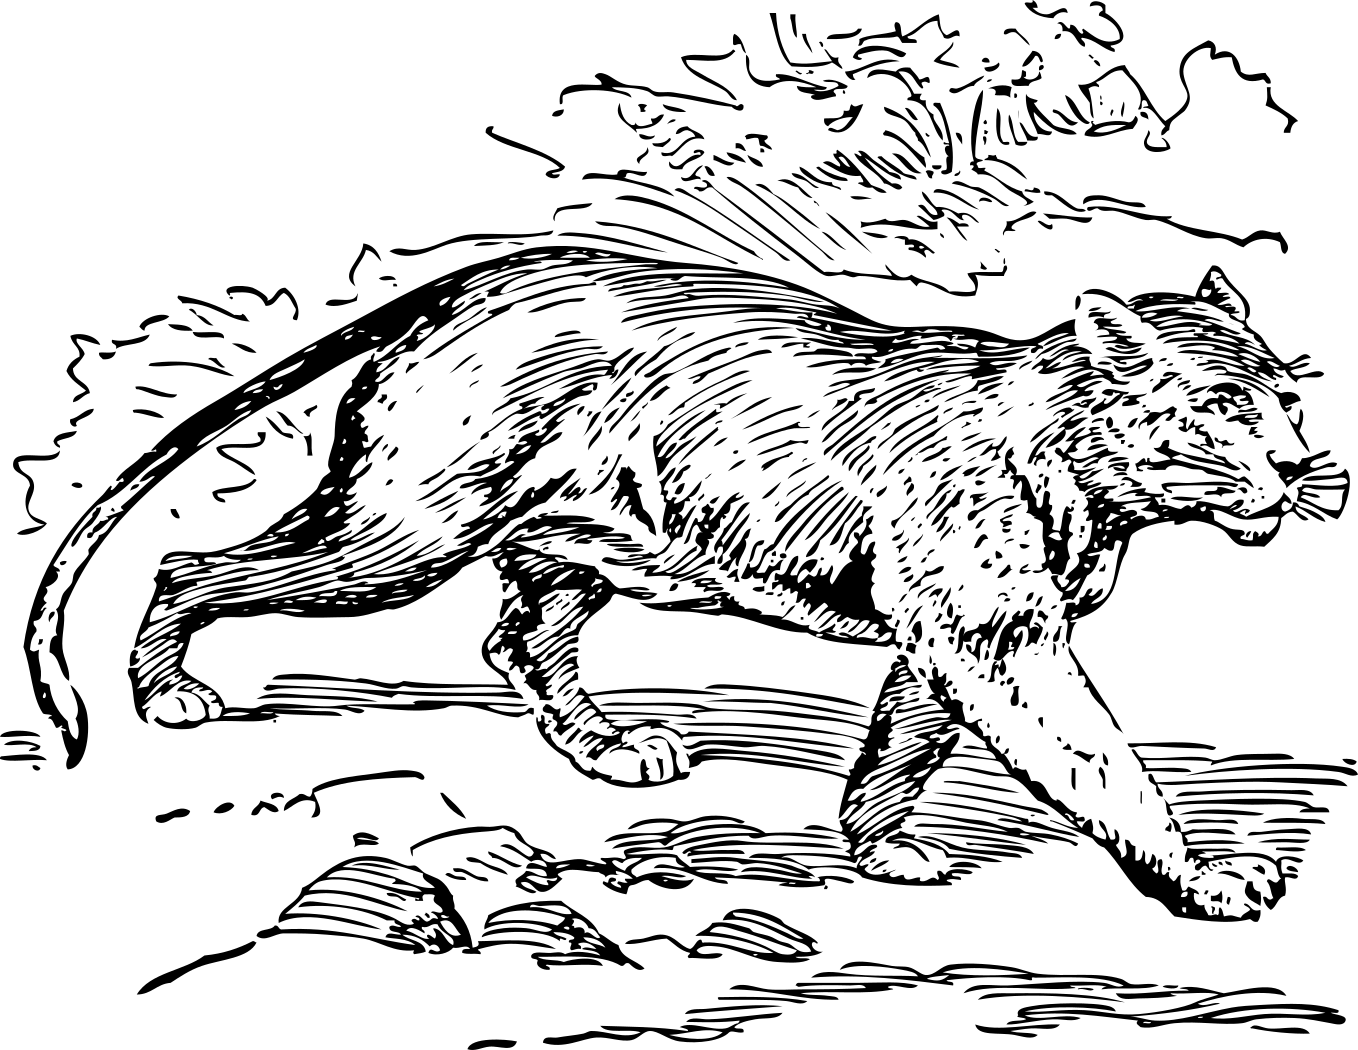
\includegraphics[width = 1\textwidth, left]{../pictures/cheetah.png}
            \end{subfigure}
            \begin{subfigure}{0.5\textwidth}
                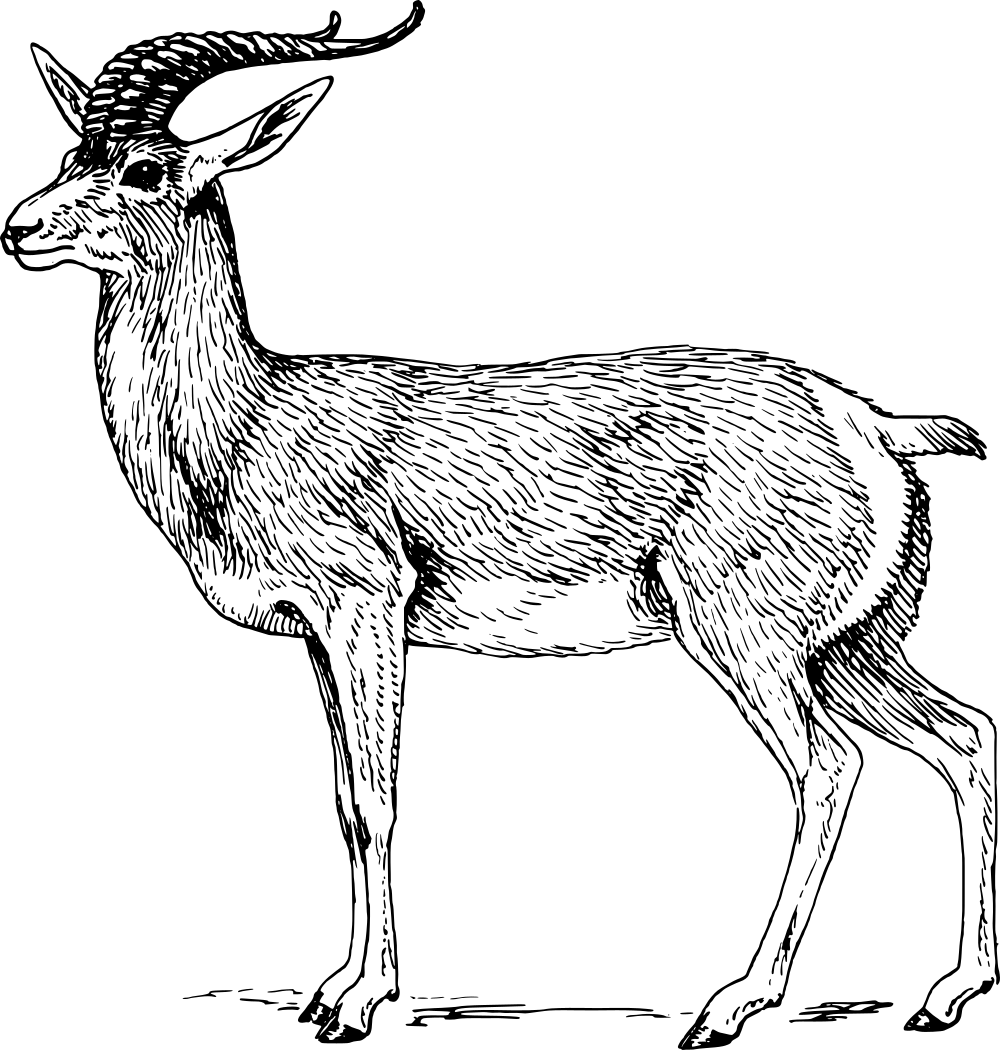
\includegraphics[width = 0.73\textwidth, right]{../pictures/gazelle.png}
            \end{subfigure}
            \caption{Illustration eines Geparden und einer Gazelle \label{fig:gazelleAndGepard}}
        \end{figure}
        \noindent
        Sei unser Gepard durch seine Geschwindigkeit den Gazellen überlegen, dann wird die Gazellenherde über Zeit in ihrer Anzahl sinken. Dabei werden die langsamen Gazellen dem Geparden erliegen und die Schnelleren überleben. Dieser Schritt wird als \textbf{Selektion} bezeichnet. Die Überlebenden werden sich fortpflanzen und mit hoher Wahrscheinlichkeit Gazellen-Babies bekommen die ähnlich schnell sind. Diesen Vorgang bezeichnen wir als \textbf{Kreuzung}. Mit welcher Wahrscheinlichkeit jedes einzelne Tier vor dem Geparden entwischen kann nennen wir \textbf{Fitness}.\\
        \\
        Jede Gazelle, oder auch \textbf{Individuum} genannt, hat eine eigene Fitness, die es aber bei Geburt noch nicht weiß, da sie noch nie vor einem Geparden weglaufen musste. Erst nachdem sie einmal erfolgreich entwischt ist, können wir uns vorstellen, was ihre Fitness ist.\\
        \\
        Ganz selten wird ein Gazellen-Baby geboren, das ein etwas längere Beine hat als alle anderen, dabei hatte keiner dieses Merkmal vor ihr. Das erlaubt ihr schneller zu laufen, was für sie erstmal positiv ist. Diese Ausprägung hat jedoch den Nachteil, dass die Standhaftigkeit darunter leidet. Diese unerwartete Veränderung bei den Kindern heißt \textbf{Mutation}.\\
        \\
        Fassen wir zusammen: Nachdem jede überlebte Gazelle sich fortgepflanzt hat, bekommen wir hoffentlich wieder eine vollzähliges Herde, die wir \textbf{Population} nennen. Nach all diesen Schritten fängt der Kampf um das Überleben wieder an und geht solange, bis sich entweder Gazellen entwickeln, die dem Gepard ständig entkommen können, oder bis die gesamte Population ausstirbt.\\
        \\
        Damit haben wir die wichtigsten Begrifflichkeiten von einem genetischen Algorithmus erklärt und kommen zur Umsetzung der einzelnen Schritte.

        \subsection{Individuen}

            Ein Individuum besteht aus einer Kodierung, auch \textbf{Zustandsraum} genannt, die die aussagekräftigen Eigenschaften von ihm ausmachen. Für eine Gazelle wäre beispielweise die folgende Kodierung möglich.

            \begin{multicols}{2}
                \hfill \\[-10mm]
                \begin{table}[H]
                    \begin{center}
                    \begin{tabular}{ |l|r| } 
                        \hline
                        Höchstgeschwindigkeit    & $ 95\; \frac{km}{h}$   \\ \hline
                        Beinlänge                & $ 86\; cm          $   \\ \hline
                        Gewicht                  & $ 43\; kg          $   \\ \hline
                        Hornlänge                & $ 12\; cm          $   \\ \hline
                    \end{tabular}
                    \end{center}
                    \caption{Kodierung einer Gazelle \label{fig:gaz-encoding}}
                \end{table}

                \noindent
                Die Aufgabe von unserem GA ist ein oder mehrere Individuen zu finden, die es schaffen vor dem Geparden wegzulaufen. Da wir aber nicht wissen, ob die vorgeschlagene Kodierung gut oder schlecht ist, müssen wir Gazellen mit zufälligen Eigenschaften erstellen und dann den Algorithmus arbeiten lassen.
            \end{multicols}
            \noindent
            Das schaffen wir, indem wir Grenzen für die Kodierung festlegen und später zufällige Werte in diesen Rahmen ausprobieren.

            \begin{table}[H]
                \begin{center}
                \begin{tabular}{ |l|r|r| } 
                    \hline
                    Eigenschaft              & Minimaler Wert        & Maximaler Wert       \\ \hline
                    Höchstgeschwindigkeit    & $ 20\; \frac{km}{h}$  & $ 100\; \frac{km}{h}$ \\ \hline
                    Beinlänge                & $ 40\; cm          $  & $ 90\; cm          $ \\ \hline
                    Gewicht                  & $ 12\; kg          $  & $ 75\; kg          $ \\ \hline
                    Hornlänge                & $  0\; cm          $  & $ 35\; cm          $ \\ \hline
                \end{tabular}
                \end{center}
                \caption{Grenzen für die Kodierung \cite{wiki:gazelle} \cite{blog:gazelle}\label{fig:gazelle-bounds}}
            \end{table}
            \noindent
            % Für die Kodierung unseres Individuums eignet sich ein Array von Zahlen. Um die gesamte Population darzustellen würde ein 2-dimensionales Array reichen, wobei jedes Element ein einzelnes Individuum darstellt. \textit{(evtl Grafik)}

        \subsection{Evaluation}
            Nachdem wir unsere Gazellenpopulation erstellt haben, müssen wir sie der Natur überlassen. Dann ist es unsere Aufgabe nach einer festen Zeitspanne und sie alle wieder aufzusammeln. Dadurch finden wir heraus wie viele Gazellen überlebet haben und können diese Information den nächsten genetischen Methoden übergeben.

        \subsection{Selektion}

            Nachdem die Evaluation vorbei ist, bekommen wir die Rückmeldung welche Gazellen überlebt haben. Aus dieser Menge können wir nun einen prozentualen Betrag wählen, die Eltern sein werden. In unserer Implementierung nennen wir diesen Parameter $\alpha$. Damit versichern wir, dass nur die erfolgreichen Eigenschaften weiter in der Population erhalten bleiben und der Rest wegfällt.

        \subsection{Kreuzung}
            Die erfolgreichen Individuen wurden ausgewählt und können sich nun fortpflanzen. Dafür nehmen wir jeweils zwei Individuen und vertauschen zufällig ihre Ausprägungen.
            \\[8mm]
            \begin{multicols}{2}
                \begin{table}[H]
                    \begin{center}
                    \begin{tabular}{ |r| } 
                        \hline
                        \hfill Eigenschaften  \\ \hline
                        \cellcolor{blue!25} $ 56\; \frac{km}{h}$ \\ \hline
                        \cellcolor{blue!25} $ 42\; cm          $ \\ \hline
                        \cellcolor{blue!25} $ 51\; kg          $ \\ \hline
                        \cellcolor{blue!25} $ 10\; cm          $ \\ \hline
                    \end{tabular}
                    \end{center}
                    \caption{Kodierung des Vaters \label{fig:enc-dad}}
                \end{table}

                \begin{table}[H]
                    \begin{center}
                    \begin{tabular}{ |r| } 
                        \hline
                        \hfill Eigenschaften  \\ \hline
                        \cellcolor{yellow!25} $ 62\; \frac{km}{h}$ \\ \hline
                        \cellcolor{yellow!25} $ 55\; cm          $ \\ \hline
                        \cellcolor{yellow!25} $ 49\; kg          $ \\ \hline
                        \cellcolor{yellow!25} $  8\; cm          $ \\ \hline
                    \end{tabular}
                    \end{center}
                    \caption{Kodierung der Mutter \label{fig:enc-mom}}
                \end{table}

            \end{multicols}

            \begin{multicols}{2}
                \begin{table}[H]
                    \begin{center}
                    \begin{tabular}{ |r| } 
                        \hline
                        \hfill Eigenschaften  \\ \hline
                        \cellcolor{blue!25}   $ 56\; \frac{km}{h}$ \\ \hline
                        \cellcolor{yellow!25} $ 55\; cm          $ \\ \hline
                        \cellcolor{yellow!25} $ 49\; kg          $ \\ \hline
                        \cellcolor{blue!25}   $ 10\; cm          $ \\ \hline
                    \end{tabular}
                    \end{center}
                    \caption{Kodierung vom Kind Nr.1 \label{fig:child-1}}
                \end{table}


                \begin{table}[H]
                    \begin{center}
                    \begin{tabular}{ |r| } 
                        \hline
                        \hfill Eigenschaften  \\ \hline
                        \cellcolor{yellow!25} $ 62\; \frac{km}{h}$ \\ \hline
                        \cellcolor{blue!25}   $ 42\; cm          $ \\ \hline
                        \cellcolor{blue!25}   $ 51\; kg          $ \\ \hline
                        \cellcolor{yellow!25} $  8\; cm          $ \\ \hline
                    \end{tabular}
                    \end{center}
                    \caption{Kodierung vom Kind Nr.2 \label{fig:child-2}}
                \end{table}
            \end{multicols}
            \noindent
            Das können wir nun sooft machen wie wir Eltern finden, oder bis wir genug Kinder produziert haben.

            \newpage
            In unserem Beispiel haben wir die Kinder mit dem folgenden Python-Code konstruiert:
            \hfill \\
            \begin{mdframed}
            \begin{minted}[escapeinside=||, linenos]{python}
vater  = [56,42,51,10]
mutter = [62,55,49,8]
kind1  = []
kind2  = []
for i in range(kodierung.length):
    r = random.uniform(0,1)
    if (r > 0.5):
        kind1[i] = vater[i]
        kind2[i] = mutter[i]
    else:
        kind1[i] = mutter[i]
        kind2[i] = vater[i]
            \end{minted}
            \end{mdframed}
            \hfill \\[4mm]
            \noindent
            In \textit{Z.1-2} definieren wir die Eigenschaften der Mutter und des Vaters. Dann iterieren wir durch die Länge der Kodierung (\textit{Z.5}) und wählen mit einer 50\% Wahrscheinlichkeit (\textit{Z.6-7}) aus für jedes Kind aus, ob die gewählte Eigenschaft vom Vater oder von der Mutter kommt.\\

            \noindent
            Diese Art und Weise zwei Individuen zu kreuzen nennt sich \textbf{n-point crossover}, weil wir die Kodierung an zufällig vielen Stellen unterbrechen. Es gibt noch andere Kreuzungsmethoden die eine eine feste Anzahl von Aufteilungen benutzen, wie \textbf{one-} oder \textbf{two-point crossover}. \\
            \\
            \noindent
            Um einen Unterschied zwischen diesen Methoden zu erkennen, stellen wir uns vor dass die Beinlänge im Zusammenhang mit der Höchstgeschwindigkeit steht, weil längere Beine eine größere Sprungweite ermöglichen. Wenn nun ein Kind gezeugt wird, dass lange Beine vererbt, wird die Höchstgeschwindigkeit dadurch nicht automatisch angepasst. Deshalb wäre es besser, wenn diese Ausprägungen zusammen übernommen werden, weil dadurch eine höhere Fitness garantiert werden kann. Kreuzungsmethoden wie n-point-crossover verletzen diese Eigenschaft eher als wie one-point-crossover.\\
            \\
            \noindent
            Je nach Implementierung verwendet man nur eins der beiden Kinder, weil das die Varianz der Gesamtpopulation weniger beeinflusst und trotzdem keinerlei Information verloren geht, weil die Eltern die Kodierung weiter tragen.

\newpage
        \subsection{Mutation}
%            ``Mutation ist hilfreich um die Varianz der Population etwas zu erhöhen'' \\
            Nachdem die Kinder erstellt wurden, müssen wir die Kodierung der Individuen etwas verändern, damit die Varianz in der Gesamtpopulation erhöht wird. Das machen wir indem wir durch die Kodierung der Kinder durchgehen und jede Ausprägung mit einer geringen Wahrscheinlichkeit verändern. Diese nennen wir $\beta$.

            \hspace*{-2cm}
            \begin{multicols}{2}
                \begin{table}[H]
                    \begin{center}
                    \begin{tabular}{ |r| } 
                        \hline
                        \hfill Eigenschaften  \\ \hline
                        \cellcolor{yellow!25} $ 62\; \frac{km}{h}$ \\ \hline
                        \cellcolor{blue!25}   $ 42\; cm          $ \\ \hline
                        \cellcolor{blue!25}   $ 51\; kg          $ \\ \hline
                        \cellcolor{yellow!25} $  8\; cm          $ \\ \hline
                    \end{tabular}
                    \end{center}
                    \caption{Kodierung von einem Kind \label{fig:child-enc}}
                \end{table}

                \begin{table}[H]
                    \begin{center}
                    \begin{tabular}{ |r| } 
                        \hline
                        \hfill Eigenschaften  \\ \hline
                        \cellcolor{yellow!25} $ 62\; \frac{km}{h}$ \\ \hline
                        \cellcolor{blue!25}   $ 42\; cm          $ \\ \hline
                        \cellcolor{red!25}    $ 45\; kg          $ \\ \hline
                        \cellcolor{yellow!25} $  8\; cm          $ \\ \hline
                    \end{tabular}
                    \end{center}
                    \caption{Mutierte Kodierung vom Kind\label{fig:mut-child-enc}}
                \end{table}
            \end{multicols}

            Die Mutation kann folgendermaßen in Python umgesetzt werden:
            \begin{mdframed}
            \begin{minted}[escapeinside=||, linenos]{python}
kinder = [k1, k2...]
beta   = 0.1
for i in range(kinder.length):
    for j in range(kodierung.length):
        r = random.uniform(0,1)
        if (r > beta):
            kinder[i][j] = sampleNewFrom(kodierung[j].range)
            \end{minted}
            \end{mdframed}
            \hfill \\[1mm]
            \noindent
            In \textit{Z.1-2} definieren wir Mutationswahrscheinlichkeit und die Kinder. Dann gehen wir jede Kodierung von jedem Kind durch (\textit{Z.3-4}) und verändern die Eigenschaft mit einer 10\% Wahrscheinlichkeit (\textit{Z.5-7}).\\

            \noindent
            Dieser Schritt ist wichtig, sodass trotz konvergierter Population neue Eigenschaften ausprobiert werden, da sie vielleicht eine bessere Lösung bieten. Der GA tendiert oft dazu sich erstmal für eine suboptimalen Lösung zu entscheiden und die Mutation erlaubt uns einen Ausweg daraus. \\

            \noindent
            In manchen Fällen kann man die Mutation noch weiter parametrisieren, indem man ein Veränderungsfaktor als Argument hinzufügt. Diese Technik benutzt man, wenn die Kodierung nicht trivialerweise verändert werden kann, da sonst bestimmte Eigenschaften verloren gehen. In Kapitel 3 wird genau so ein Fall besprochen, weil wir unsere Individuen durch eine Wahrscheinlichkeitsverteilung darstellen. 

\newpage

        \subsection{Repopulation}
            Die Eltern wurden ausgewählt, die Kindern gezeugt und mutiert, nun müssen wir die Population in eine Form bringen, sodass die Evaluation neu gestartet werden kann. Wir stellen das Problem wieder an einem Beispiel dar.\\

            \begin{mdframed}
            \begin{minted}[escapeinside=||, linenos]{python}

population = [i1,i2,...]                  # population.length = 10
alpha      = 0.4
eltern     = selection(population, alpha) # eltern.length = 4
kinder     = crossover(eltern)            # kinder.length = 4
beta       = 0.1
mutkinder  = mutation(kinder, beta)       # mutkinder.length = 4

newpopulation = eltern + mutkinder        # newpopulation.length = 8
            \end{minted}
            \end{mdframed}
            \hfill \\
            \noindent
            Wir sehen dass uns zwei Individuen weniger als zu Anfang haben können deshalb die Evaluation nicht neu starten. Dieses Problem kann man auf viele Weisen angehen, die ihre eigenen Vorteile und Nachteile haben. 

            \subsubsection*{Mehr Kinder erstellen}
                Es ist möglich während der Kreuzung solange Kinder zu erzeugen, bis die Population wieder ihre Ausgangsgröße angenommen hat. Ein Vorteil wäre, dass diese Individuen mit wahrscheinlich besseren Ausgangskodierungen starten als Neue. Der Nachteil ist jedoch die gesenkte Varianz in der Population und die erhöhte Wahrscheinlichkeit zum Feststecken in einem suboptimalen Lösungen.

            \subsubsection*{Nicht selektiere Individuen nachfüllen}
                Man kann die nicht benutzen Individuen aus der vorherigen Population zum Auffüllen benutzen, was sich aber nur dann gewählt werden sollte, wenn die Chance bestünde, dass sie in der erneuten Simulation besser abschneiden als bisher. Ansonsten nehmen sie den Platz für ein potenziell besseres Individuum weg.

            \subsubsection*{Neue Individuen erstellen}
                In unserer Implementierung haben wir uns für das Nachfüllen von völlig neuen Individuen entschieden, da dadurch die Varianz der Population angehoben wird und dadurch mehr Lösungen möglich sind. Ein Nachteil ist dabei sind die potenziellen Kinder die  keinen Platz bekommen, aber da dadurch keine Information verloren geht, können wir es vernachlässigen.
\newpage

    \section{Neuroevolution}
%        ``Neuroevolution beschäftigt sich mit der Verknüpfung von Genetischen Algorithmen und Neuronalen Netzn''
        Der Begriff der Neuroevolution wurde im Jahre 1988 von D. Whiteley \cite{whiteley88} als alternative Möglichkeit zum Trainieren von künstlichen neuronalen Netzen (\textbf{KNNs}) vorgeschlagen. Dabei wird versucht aus der Synergie von dem \textbf{selbstlernenden Charakter} von KNNs und der \textbf{explorativen Suche} eines GAs eine Taktik oder ein Klassifikator zu entwickeln der völlig neue Lösungen finden kann. Den Beweis dafür hat man bereits im Jahr 1995 am Spiel \textit{Othello} festgestellt. \cite{othello95} \\[2mm]
        \noindent
        Wir versuchen in diesem Kapitel einen groben Überblick über die Funktionsweise von KNNs zu verschaffen und stellen den Bezug zu genetischen Algorithmen dar. Eine weitaus formalere Erklärung findet sich im Paper von ....

        \subsection{Künstliche neuronale Netze}

            Die Idee hinter künstlichen neuronalen Netzen ist der Versuch die Struktur vom menschliche Gehirn nachzuahmen. Ein übliches KNN besteht jedoch aus vielfach weniger Neuronen, meist hundert bis mehrere tausend, wobei unser Gehirn 86 Milliarden\cite{brainsize} besitzt.\\
            \noindent
            Ein künstliches Neuron kann man sich anschaulich als eine Formel vorstellen, die \textbf{eine oder mehrere Eingaben} über \textbf{gewichtete Pfade} bekommt, sie \textbf{aufsummiert} und eine Aktivierungsfunktion auf das Ergebnis anwendet, die auf den Bereich $[0,\infty]$, $[0,1]$, oder $[-1,1]$ abbildet. Dieses Resultat nennen wir $\hat{y}$:

            \begin{figure}[H]
                \begin{mdframed}
                    \noindent
                    Sei $n$ die Anzahl der Eingaben,\\
                    \hspace*{4.5mm}    $X = \{x_0,x_1,...,x_n\}$ die Eingabe,\\
                    \hspace*{4.5mm}    $W = \{w_0, w_1,...,w_n\}$ die jeweiligen Gewichte, \\
                    \hspace*{4.5mm}    $\sigma(x) = max(x,0)$ als Aktivierungsfunktion:\\[4mm]
                    \hspace*{50mm} \Resize{4.5cm}{$\widehat{y} = \sigma(\sum^{n}_{i = 0} x_i \cdot w_i)$}
                \end{mdframed}
                \caption{\label{neuron-math} Formel zur Berechnung des Ergebnisses eines Neurons}
            \end{figure}

            \noindent
            Wenn man nun mehrere von diesen Neuronen in Reihe zusammenschaltet (Abbildung \ref{fig:nntikz}), kriegt man ein vollständig vermaschtes Netz, welches grundsätzlich in drei Schichten unterteilt werden kann.
            \begin{itemize}
                \setlength{\itemsep}{5pt}
                \item \textbf{Eingabeschicht} \\
                    Hier kommt der Ausgangszustand rein, sei es ein kodierter Zustand eines Spiels, RGB Werte von einem Bild, oder der DAX.
                \item \textbf{Versteckte Schicht(en)} \\
                    Dieser Teil des Netzes besteht oft aus mehreren Schichten, da er für die Abstraktion und die Lernfähigkeit verantwortlich ist \cite{ANNModeling}. Er bekommt die Signale aus der Eingabeschicht, die er verarbeitet und weiterleitet. Je nachdem, welche Neuronen dabei \textit{feuern}, beeinflusst das Endergebnis stark.
                \item \textbf{Ausgabeschicht} \\
                    Die Ausgabeschicht ist oft zum Sammeln der Signale von der vorherigen Schicht zuständig und auf ihren Ergebnissen wird dann eine \textbf{Aktivierungsfunktion} angewendet, die die kumulierten Resultate in eine passende Form bringt. Sie varrieren zwischen einfachen Ja/Nein Aussgagen, oder wie wir später kennen lernen werden, auch Wahrscheinlichkeitsverteilungen.

            \end{itemize}

            \tikzset{%
              input neuron/.style={
                circle,
                draw,
                minimum size=1cm,
                fill=inputnode
              },
              hidden neuron/.style={
                circle,
                draw,
                minimum size=1cm,
                fill=hiddennode
              },
              output neuron/.style={
                circle,
                draw,
                minimum size=1cm,
                fill=outputnode
              },
              neuron missing/.style={
                draw=none, 
                scale=1.97,
                text height=0.333cm,
                execute at begin node=\color{black}$\vdots$,
                fill=missingnode
              },
              perceptron/.style={
                circle,
                draw,
                scale=3,
                minimum size=1cm,
                fill=perceptronnode
              }
            }

            \begin{figure}[H]
            \centering
                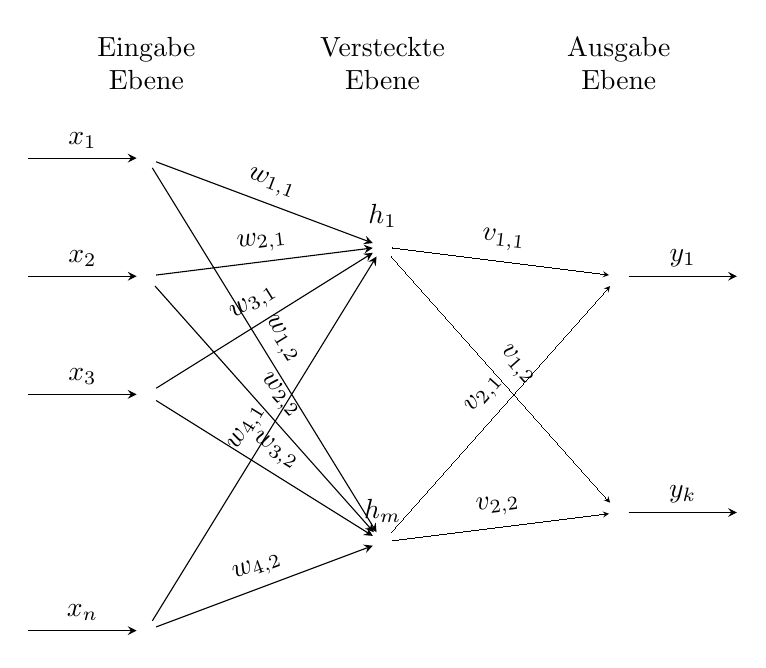
\begin{tikzpicture}[x=1.5cm, y=1.5cm, >=stealth]
                    \foreach \m/\l [count=\y] in {1,2,3,missing,4}
                        \node [input neuron/.try, neuron \m/.try] (input-\m) at (0,2.5-\y) {};
                    \foreach \m [count=\y] in {1,missing,2}
                        \node [hidden neuron/.try, neuron \m/.try ] (hidden-\m) at (2,2-\y*1.25) {};
                    \foreach \m [count=\y] in {1,missing,2}
                        \node [output neuron/.try, neuron \m/.try ] (output-\m) at (4,1.5-\y) {};
                    \foreach \l [count=\i] in {1,2,3,n}
                        \draw [<-] (input-\i) -- ++(-1,0)
                            node [above, midway] {$x_\l$};
                    \foreach \l [count=\i] in {1,m}
                        \node [above] at (hidden-\i.north) {$h_\l$};
                    \foreach \l [count=\i] in {1,k}
                        \draw [->] (output-\i) -- ++(1,0)
                            node [above, midway] {$y_\l$};
                    \foreach \i [count=\n] in {1,...,4}
                        \foreach \j [count=\m] in {1,...,2}
                            \draw [->] (input-\i) -- node [sloped, above] {$w_{\n,\m}$} (hidden-\j);
%                            \ifthenelse{\n=1}{
%                                \draw [->] (input-\i) -- node [midway, sloped, above=0.3mm] {$w_{\n,\m}$} (hidden-\j);
%                            }{
%                                \draw [->] (input-\i) -- (hidden-\j);
%                            }
                    \foreach \i [count=\n] in {1,...,2}
                        \foreach \j [count=\m] in {1,...,2}
                            \draw [line width = 0.0mm, ->] (hidden-\i) -- node [midway, sloped, above=0.3mm] {$v_{\n, \m}$} (output-\j);
                    \foreach \l [count=\x from 0] in {Eingabe, Versteckte, Ausgabe}
                        \node [align=center, above] at (\x*2,2) {\l \\ Ebene};
                \end{tikzpicture}
                \caption{Skizze von einem vollständig vermaschten künstlichen neuronales Netz \label{fig:nntikz}}
            \end{figure}
            \noindent
            Neuronen wie in Abbildung \ref{fig:nntikz} zusammen zu verknüpfen nennt sich ein \textbf{Feedforward} Netzwerk, da es keine Zyklen beinhaltet. Sie besitzen die Einschränkung das sie ohne Rücksicht auf die resultierenden Effekte in der Domäne ein Ergebnis liefern, da sie das Signal nur nach vorne weiterleiten.\\

            \noindent
            Um eigene Resultate und zeitliche Abstraktionen einfacher zu berücksichtigen gibt es \textbf{rekurrente Netze} die direkte Zyklen beinhalten.

            \subsubsection*{LSTM Ebene}
                Ein spezielles Neuron aus dem rekurrente Netze bestehen können, ist das \textbf{Long Short Term Memory} (LSTM) Neuron\cite{lstm}. Es zeichnet sich durch die Eigenschaft aus, dass es über lange Zeitfenster Information behalten kann. Der Aufbau basiert auf dem Modell einer Speicherzelle, sodass wir durch verschiedene Eingänge (\textbf{Gates}), die Schreib-,Lese- und Reset-Aktionen nachbauen können \cite{lstm-new}. Einer der wichtigste Aspekte von diesen Neuronen ist jedoch, dass sie ableitbar sind, weil dadurch die Trainingsmethode \textbf{Backpropagation} ermöglicht wird \cite{backprop}.

\newpage
            \subsubsection*{Backpropagation}
                Um diese Technik zum Trainieren von KNNs zu erklären müssen wir zunächst zeigen wie man den Fehler von einem neuronalen Netz misst. Dafür brauchen wir eine \textbf{Kostenfunktion} die uns die Abweichung zum Soll-Ergebnis gibt. Die Ergebnisse des Netzes für $\widehat{y}$ ist in Abbildung \ref{neuron-math} definiert.

                \begin{figure}[H]
                    \begin{mdframed}
                        \noindent
                        Sei $m$ die Größe des Trainingssets,\\
                        \hspace*{4.5mm} $Y = \{y_0, y_1,...,y_m\}$ ein Vektor von Soll-Ergebnissen, \\
                        \hspace*{4.5mm} $\widehat{Y} = \{\widehat{y}_0, \widehat{y}_1,...,\widehat{y}_m\}$ ein Vektor von Resultaten des KNNs, dann ist:\\[4mm]
                        \hspace*{30mm} \Resize{7cm}{cost$(Y, \widehat{Y}) = \frac{1}{m} \cdot \sum_{j = 0}^{m} \; (y_j - \widehat{y}_j)^2$}\\[4mm]
                        die mittlere quadratische Abweichung.
                    \end{mdframed}
                    \caption{\label{cost-math} Formel zur Berechnung des \textit{MSE} Fehlers von einem KNN}
                \end{figure}
                \noindent
                Eine der möglichen Kostenfunktionen sieht man in Abbildung \ref{cost-math}, die \textbf{mittlere quadratische Abweichung} (MSE). Je kleiner diese Kostenfunktion ist, umso besser kann unser KNN die Ergebnisse nachahmen. Um die Kosten zu minimieren, müssen wir die gesamte Funktion samt der Berechnung vom $\widehat{y}$ partiell nach den Gewichten ableiten. \\[2mm]
                Mit dem resultierenden Gradienten verändern wir die Gewichte, sodass der Fehler möglichst verringert wird. Dafür leiten wir die Anpassungsformel für jedes Gewicht her:

%                 Damit finden wir heraus, wie wir jedes einzelne Gewicht verändern müssen damit am Ende das richtige Ergebnis rauskommt, sodass alles gegen 0 geht. Dafür leiten wir die Anpassungsformel für jedes Gewicht her:

                \begin{figure}[H]
                    \begin{mdframed}
                        \noindent
                        Pro Beobachtung $j$ in $Y$,\\
                        pro Gewicht $i$ in $W$ leiten wir partiell nach $w_i$ ab:\\[4mm]
    \hspace*{40mm} \Resize{5.5cm}{$\frac{\partial \text{cost}(y_j,\widehat{y}_j)}{\partial w_i} = \frac{\partial}{\partial w_i} (y_j - \widehat{y}_j)^2$} \\[2mm]
    \hspace*{62.3mm} \Resize{7.0cm}{$ = \frac{\partial}{\partial w_i} (y_j - max(\sum_{i = 0}^{n} x_i \cdot w_i ,0))^2$} \\[2mm]
    \hspace*{62.3mm} \Resize{6.25cm}{$ = -2 \cdot \frac{\partial}{\partial w_i} \; max(\sum_{i = 0}^{n} x_i \cdot w_i ,0)$} \\[2mm]
    \hspace*{62.3mm} \Resize{6.25cm}{$ =   \begin{cases}
                                            0 & \sum_{i = 0}^{n} x_i \cdot w_i < 0 \\[2mm]
                                            -2 \cdot x_i & \sum_{i = 0}^{n} x_i \cdot w_i > 0 \\
                                        \end{cases}$}\\[4mm]
                        Damit bekommen wir für Anpassungsregel für jedes Gewicht:\\[4mm]
                        \hspace*{40mm} \Resize{6.5cm}{$w_i \leftarrow w_i + \begin{cases}
                                                                               0 & \sum_{i = 0}^{n} x_i \cdot w_i < 0 \\[2mm]
                                                                               -2 \cdot x_i & \sum_{i = 0}^{n} x_i \cdot w_i > 0 \\
                                                                             \end{cases}$}
                    \end{mdframed}
                    \caption{\label{derivative} Berechnung der Anpassungsregel für jedes Gewicht nach MSE}
                \end{figure}


                \noindent
                Diese Technik kann man benutzen, solange das gesamte Netz als Formel dargestellt ableitbar ist, selbst wenn es mehrere versteckte Schichten hat. Leider braucht sie dafür ein Trainingsset von Daten, was in oft aufwendig zu generieren ist. Deshalb benutzen wir eine simulationsbasierte Lernmethode.


            \subsubsection*{Softmax Ebene}
                Es gibt eine Aktivierungsfunktion der wir besondere Aufmerksamkeit widmen, da sie die Neuronen der Ausgabeschicht zu einem nützlichen Ergebnis zusammenfassen kann. Die generalisierte logistische Funktion, oder auch \textbf{normalisierte Exponentialfunktion} nimmt als Argument einen $k$-dimensionalen Vektor \textbf{z} von reelen Zahlen und gibt uns widerrum den gleichen Vektor zurück, wo alle Werte auf den Bereich [0,1] normalisiert wurden.

            \begin{figure}[H]
                \begin{mdframed}
                    Sei $j = 1,2,...,K$: \\
                    \hspace*{45mm} \Resize{4cm}{$\sigma(\textbf{z})_j = \frac{e^{\textbf{z}_j}}{\sum^{K}_{k = 1} e^{\textbf{z}_k}}$}
                \end{mdframed}
                \caption{\label{softmax} Definition der Softmax Funktion}
            \end{figure}

            \noindent
            Aufmerksame Leser fragen sich vielleicht warum man keine einfache Normalisierung vornimmt. Wenn man als Trainingsfunktion bei Backpropagation den logistischen Fehler (\textbf{logistic-loss}) oder \textbf{cross entropy loss} benutzt, kürzt sich das $e$ weg und bietet sich daher an.

        \subsection{Verbindung mit genetischen Algorithmen}
            Wenn wir nun zum Trainieren von ANNs genetische Algorithmen benutzen wollen, müssten wir das Netz als Liste von Gewichten kodieren, aus denen es besteht. Ein Beispiel dafür bietet der \textbf{GENITOR}\cite{moriarty1999evolutionary} Algorithmus. Dabei werden die einzelnen Gewichte der Kreuzung und einer speziellen Mutation ausgesetzt die von der Varianz der Gesamtpopulation abhängt. \\

            \noindent
            Ein weiterer Ansatz ist \textbf{SANE}\cite{moriarty1999evolutionary}, der einzelne Neuronen für die \textit{Hidden Ebene} entwickelt und daraus ein Netz generiert. Dadurch wurde die Mobility-Strategie für das Spiel Othello wiederentdeckt. \\

            \noindent
            Leider benutzen neuronale Netze heutzutage je nach Anwendungsgebiet immer aufwendigere Strukturen die extrem viele Gewichte besitzen. Eine naive genetische Suche in so einem hochdimensionalen Zustandsraum dauert zu lange und deshalb gibt es Techniken die uns erlauben zielsicherer und effizienter den Raum aller Möglichkeiten zu durchsuchen.

%            ``Die Verknüpfung findet in der Kodierung von den Individuen statt - wir nehmen eine (naive) Darstellung von allen Gewichten''
%            ``Problematik -> Folgerung zu DCT''

    \section{Diskrete Kosinus Transformation}
        % ``Der Suchraum kann durch die sog. DCT auf beliebige Dimensionalität eingeschränkt werden, wenn bestimmte Annahmen getroffen werden können'' \\
        % ``Fouriertransformationen machen folgendes...'' \\
        % ``Es gibt eine Inverse die aus einem n-stelligen liste eine m-stellige macht, wo die Zahlen korelliert sind (Beispiele)''

        Eine dieser Techniken ist die Nutzung der diskreten Kosinustransformation (\textbf{DCT}), die zur Familie der Fouriertransformationen gehört. Eine \textbf{Fouriertransformation} spaltet ein Signal in beliebig viele trigonometrische Funktionen, wie Sinus oder Kosinus und über die Summe dieser Funktionen kann jede mögliche Ausprägung von Daten beschrieben werden. \\

        \noindent
        Diese Fouriertransformation liefert uns dadurch ein diskretes Frenquenzenspekturm, das in Form von Koeffizienten dargestellt wird. Dabei wird pro kodierter Datenpunkt ein Koeffizient benutzt. Um die Daten wiederherzustellen gibt es die inverse Kosinustransformation die die Koeffizienten wieder umwandelt.

        \begin{multicols}{2}
            \begin{figure}[H]
                \begin{center}
                    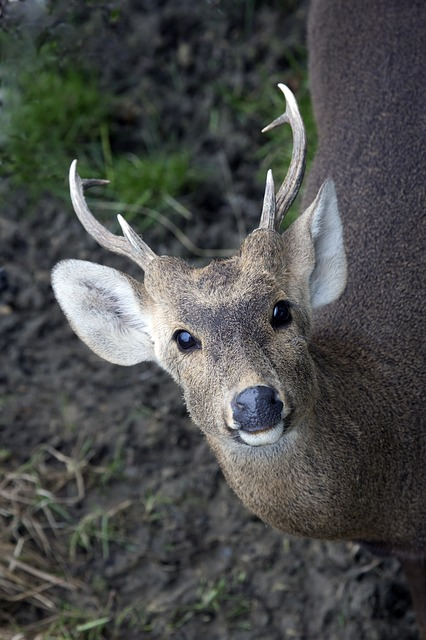
\includegraphics[scale=1]{../pictures/gazelle-uncompressed.jpg}\\
                    \caption{Unkomprimiert}\label{fig:gazelle-uncompressed}
                \end{center}
            \end{figure}
            \par
            \begin{figure}[H]
                \begin{center}
                    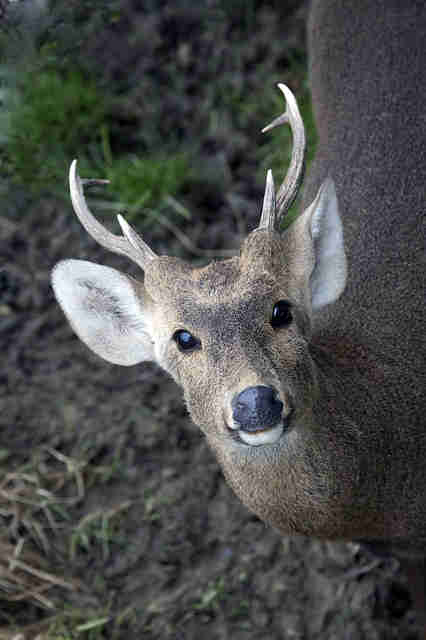
\includegraphics[scale=0.239]{../pictures/gazelle-compressed.jpg}\\
                    \caption{Komprimiert (1:5)}\label{fig:gazelle-compressed}
                \end{center}
            \end{figure}
        \end{multicols}

        \noindent
        Wenn wir viele der Koeffizieten nicht benutzen und trotzdem versuchen die Datenpunkte wiederherzustellen, kriegen wir lediglich eine Annäherung, wie man in Abbildung \ref{fig:gazelle-compressed} sieht. Sie ist meistens aber so gut genug, dass wir keinen Unterschied merken. Eine sehr ähnliche Kompressionsmethode kennt man aus dem Bildformat JPEG oder dem Videoformat MPEG.

        \subsection{Kodierung des Suchraums}

            Diese Technik wenden wir nun auf die Gewichte von unserem neuronalen Netz an. Dafür beschränken wir den Suchraum auf eine kleine Anzahl der Koeffizienten und benutzen die inverse Kosinustransformation um aus ihnen die nötige Anzahl von Gewichten zu erstellen. In Abbildung \ref{fig:dct-pre},\ref{fig:dct-after} sieht man eine Anwendung auf 100 Gewichte die in einem Verhältnis von 1:2 komprimiert wurden. Das bedeutet dass wir den Suchraum mit dem sichtbaren Genauigkeitsverlust halbiert haben.\\

            \noindent
            Bei größeren Verhältnissen bemerken wir eine starke örtliche Korrelation (\ref{fig:dct-my-case}) zwischen den benachbarten Zahlen und diese Eigenschaft passt zu der Annahme dass sich Gewichte in neuronalen Netzen ähnlich verhalten. Eine ausführlichere Erklärung findet sich im Ursprungspaper für die Anwendung in der Neuroevolution.\cite{cosyne1}
            \begin{multicols}{2}
                \begin{figure}[H]
                    \begin{center}
                        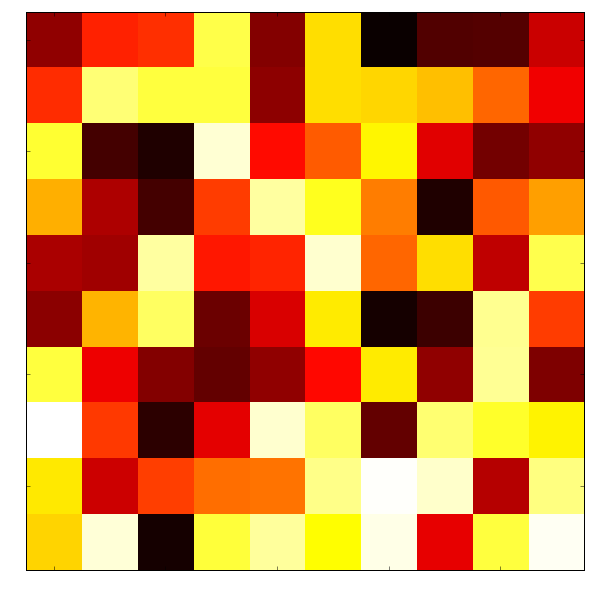
\includegraphics[scale=0.2]{../pictures/DCT-pre.png}\\
                        \caption{Unkomprimiert}\label{fig:dct-pre}
                    \end{center}
                \end{figure}
                \par
                \begin{figure}[H]
                    \begin{center}
                        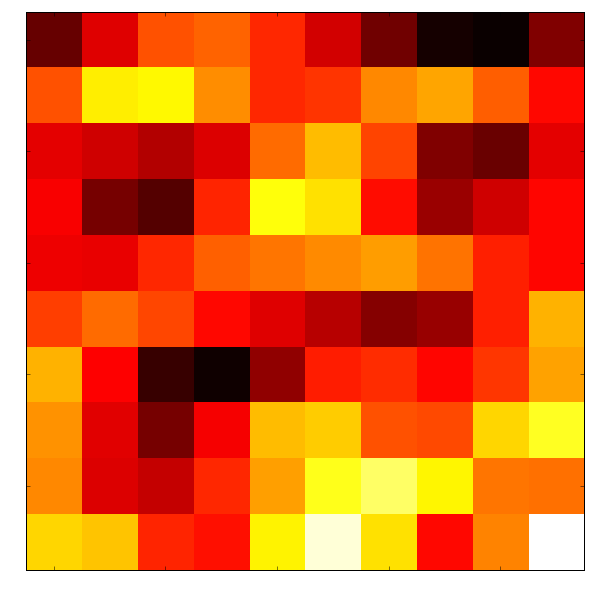
\includegraphics[scale=0.2]{../pictures/DCT-after.png}\\
                        \caption{Komprimiert (1:2)}\label{fig:dct-after}
                    \end{center}
                \end{figure}
            \end{multicols}

    \section{Cooperative Synapsen Neuroevolution}
%         ``CoSyNE wurde vom Prof.Dr.Schmidhuber an der ETH Zürich entwickelt und hat damit sehr viele anderen Algorithmen in den Schatten gestellt''\\
%        ``Methodik, ist wie GA bloß mit einer Aktion mehr die statt spielbare `Policies', nur im Koeffizientraum entwickle'' \\
%        ``Dies erlaubt eine (zitat) Kooperative Entwicklung von Koeffizienten für die nachfolgenden Inv.DCT'' \\
%        ``Kein Crossover, geringe Mutation'' \\
%        ``Beispiele vom Erfolg'' \\
        Nachdem wir den Zustandsraum komprimiert haben, sodass ein genetischer Algorithmus ihn in absehbarer Zeit entwickeln und ein neuronales Netz befüllt werden kann, erschließt sich die Verküpfung zu einem mächtigen Werkzeug das viele interessante Eigenschaften besitzt. Dieser Algorithmus wird \textbf{Cooperative Synapsen Neuroevolution}\cite{cosyne2}, oder auch \textbf{CoSyNE} genannt.\\

        \noindent
        Er zeichnet sich speziell dadurch aus, dass er auf kontinuierlichen Zuständen und Aktionen funktioniert und spärliche Fitnessignale interpretieren kann. Das schafft er indem er rekurrente Netze aufbaut und die genetische Suche mit aggresiver Mutation im Zustandsraum beschleunigt. Ein gutes Beispiel dafür ist das Rennspiel \textbf{TORCS}\cite{cosyne3} wo der Algorithmus 993 Gewichte in 33 Koeffizienten kodiert \textit{(Faktor 1:30)} und lediglich durch die Bilddaten ähnlich gute Ergebnisse liefert wie die per Hand programmierten Agenten die die Physik des Spieles kennen.\\

        \noindent
        Ein großer Nachteil von genetischen Algorithmen ist das sie oft schnell zu lokalen Maxima konvergieren und sehr schlecht aus diesem Tal rauskommen. Um dieses Problem anzugehen, versucht man die Stellschrauben wie Mutationswahrscheinlichkeit oder Kinderanzahl per Hand zu verändern. CoSyNE benutzt dafür eine ganz eigene \textbf{genetische Methode} um die Suche einfacher zu gestalten. Sie nennt sich Permutation und erzeugt innerhalb der gesamten Population Unterteilungen in kleinere Populationen die in einer \textbf{kooperativen und koevolutionären} Beziehung stehen.
%          \begin{figure}[H]
%              \begin{center}
%                  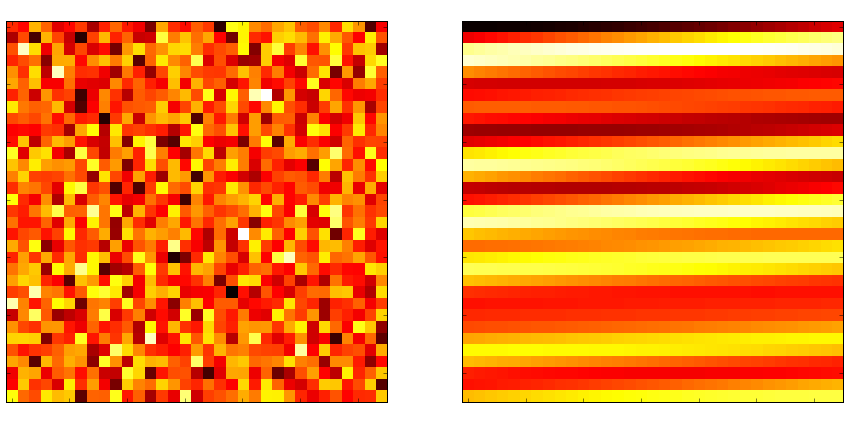
\includegraphics[scale=0.5]{../pictures/DCT-my-case.png}\\
%                  \caption{1024 Gewichte auf 23 Koeffizienten reduziert}\label{fig:dct-my-case}
%              \end{center}
%          \end{figure}
% \newpage
        \subsection{Permutation}
            % ``Wir transponieren, shuffeln und transponieren zurück''
            Der Permutationsschritt wird ganz am Ende von dem genetischen Algorithmus statt der Repopulation aufgerufen und vermischt jeden \colorbox{green!25}{Eigenschaftsraum} der Gesamtpopulation. 

            \begin{table}[H]
                \begin{center}
                \begin{tabular}{ |r|r|r|r|r| } 
                    \hline
                    Individuum & \cellcolor{green!25} Höchstgeschwindigkeit & \cellcolor{green!25} Beinlänge & \cellcolor{green!25} Gewicht & \cellcolor{green!25} Hornlänge \\ \hline
                    $1$        & $60\; \frac{km}{h}$   & $40\; cm$ & $50\; kg$ & $10\; cm$ \\ \hline
                    $2$        & $61\; \frac{km}{h}$   & $41\; cm$ & $51\; kg$ & $11\; cm$ \\ \hline
                    $3$        & $62\; \frac{km}{h}$   & $42\; cm$ & $52\; kg$ & $12\; cm$ \\ \hline
                    $4$        & $63\; \frac{km}{h}$   & $43\; cm$ & $53\; kg$ & $13\; cm$ \\ \hline
                    $5$        & $64\; \frac{km}{h}$   & $44\; cm$ & $54\; kg$ & $14\; cm$ \\ \hline
                    $6$        & $65\; \frac{km}{h}$   & $45\; cm$ & $55\; kg$ & $15\; cm$ \\ \hline
                \end{tabular}
                \end{center}
                \caption{Vor der Permutation \label{fig:pre-perm}}
            \end{table}

            \begin{table}[H]
                \begin{center}
                \begin{tabular}{ |r|r|r|r|r| } 
                    \hline
                    Individuum & \cellcolor{green!25} Höchstgeschwindigkeit & \cellcolor{green!25} Beinlänge & \cellcolor{green!25} Gewicht & \cellcolor{green!25} Hornlänge \\ \hline
                    $1$        & \cellcolor{blue!45} $61\; \frac{km}{h}$   & \cellcolor{yellow!25} $43\; cm$ & \cellcolor{red!15} $54\; kg$ & \cellcolor{violet!45} $12\; cm$ \\ \hline
                    $2$        & \cellcolor{blue!45} $60\; \frac{km}{h}$   & \cellcolor{yellow!45} $44\; cm$ &                    $51\; kg$ & \cellcolor{violet!25} $14\; cm$ \\ \hline
                    $3$        & \cellcolor{blue!15} $64\; \frac{km}{h}$   & \cellcolor{yellow!65} $45\; cm$ & \cellcolor{red!35} $53\; kg$ & \cellcolor{violet!45} $10\; cm$ \\ \hline
                    $4$        &                     $63\; \frac{km}{h}$   & \cellcolor{yellow!25} $40\; cm$ & \cellcolor{red!35} $52\; kg$ & $13\; cm$ \\ \hline
                    $5$        & \cellcolor{blue!15} $62\; \frac{km}{h}$   & \cellcolor{yellow!45} $41\; cm$ &                    $54\; kg$ & \cellcolor{violet!25} $11\; cm$ \\ \hline
                    $6$        &                     $65\; \frac{km}{h}$   & \cellcolor{yellow!65} $42\; cm$ & \cellcolor{red!15} $50\; kg$ & $15\; cm$ \\ \hline
                \end{tabular}
                \end{center}
                \caption{Nach der Permutation \label{fig:pre-perm}}
            \end{table}

            \noindent
            Wenn wir uns die Population als zweidimensionale Liste vorstellen, wo jedes Indviduum eine eigene Liste mit seinen spezifischen Ausprägungen ist, können wir die Population transponieren, wobei nun jede Eigenschaft eine eigene Liste ist, diese vermischen und wieder zurück transponieren um die neuen Individuen zu bekommen. Der folgende Pythoncode veranschaulicht das Prinzip unter Verwendung der \textit{numpy} Bibliothek.

            \begin{mdframed}
            \begin{minted}[escapeinside=||, linenos]{python}
import numpy as np

i_1 = [1,10,100,1000] # Individuum 1-5
i_2 = [2,20,200,2000]
i_3 = [3,30,300,3000]
i_4 = [4,40,400,4000]
i_5 = [5,50,500,5000]

population = np.array([i_1, i_2, i_3, i_4, i_5])
eigenschaftsraum = np.transpose(population)
  
for eig in eigenschaftsraum:
    np.random.shuffle(eig)

population = np.transpose(eigenschaftsraum)

print population
> [[   2   40  500 5000]
   [   1   50  200 1000]
   [   4   10  300 3000]
   [   3   30  100 2000]
   [   5   20  400 4000]]

            \end{minted}
            \end{mdframed}
            \noindent
            Man erkennt leicht, dass keiner der ursprünglichen Individuen erhalten bleibt und wir vollkommen Neue bekommen. Der Sinn hinter dem Verschmischen in der Eigenschaftsebene versteckt sich in der \textbf{Verknüpfungung mit der Kreuzungsmethode}. Wenn wir zwei Individuen kreuzen, werden ihre Kinder sicherlich die gesamte Information von ihren Eltern in der Population übernehmen. Da CoSyNE den Repopulationsschritt nicht ausführt, aber dennoch schlechte Individuen wegwirft, wird irgendwann nur noch die Kodierung von den Kindern übrig bleiben.\\

            \noindent
            Das führt zur Homogenität in den einzelnen Eigenschaften, die zum Beispiel dafür verantworlich ist, dass alle Individuen gleich große Hörner haben. Wenn nun innerhalb der Hornlänge zufällig gemischt wird, bleibt alles gleich, da die gesamte Liste aus dem gleichen Element besteht. \\

            \noindent
            Die Annahme von CoSyNE ist dass die Lösung für das Problem in der Kombination von den Ausprägungen von allen Individuen liegt, die wir am Anfang erstellen. Durch das aggressive Aussortieren durchsuchen wir den Raum aller Möglichkeiten schneller und darin liegt der größte Vorteil von diesem Algorithmus.

\newpage
    \section{Cross Entropy Method}
        Eine andere Möglichkeit die Individuen in dem GA zu kodieren stellt die \textbf{Cross Entropy Method} dar. Das ist ein Algorithmus der oft als Vergleichskriterium verwendet wird, da er oft zu suboptimalen Strategien konvergiert\cite{cem}. Die Anwendung in unserem neuroevolutionären Schema basiert darauf, dass wir Individuen nicht als Ansammlung von Zahlen zu speichern, sondern jede Eigenschaft als Normalverteilung dargestellt wird. Diese Abläufe illustrieren wir anhand der Erklärung für eine Normalverteilung ist.

        \subsection{Normalverteilung}

            Eine Normalverteilung ist eine sehr bekannte stetige Wahrscheinlichkeitsverteilung. Ihre Wahrscheinlichkeitsdichtefunktion wird oft Gauß-Kurve oder Glockenkurve genannt und findet Anwendung in verschiedensten Anwendungsgebieten, weil sie natürliche Vorgänge exakt oder ähnlich genug modelliert. Bekannte Beispiele dafür sind die Streuung von Messfehlern oder die irreguläre Bewegung von Partikeln in einer Flüssigkeit (\textbf{Brownsche Bewegung}).\\

            \noindent
            Die Wahrscheinlichkeitsdichtefunktion der Normalverteilung ist von zwei Parametern abhängig, dem Durchschnitt und der Standardabweichung:

            \begin{figure}[H]
                \begin{mdframed}
                    \noindent
                    Sei $\mu$ der Durchschnitt,\\
                    \hspace*{4.5mm}    $\sigma$ die Standardabweichung, dann ist\\[4mm]
                    \hspace*{50mm} \Resize{6cm}{$\mathcal{N}(x\;|\;\mu, \sigma^2) = \frac{1}{\sqrt{2\pi\sigma^2}} \cdot e^{-\frac{(x - \mu)^2}{2\sigma^2}} $} \\[4mm]
                    \hspace*{4.5mm} die Wahrscheinlichkeitsdichtefunktion der Normalverteilung.
                \end{mdframed}
%                \caption{\label{norm-dist-pdf-formel} Definition der Wahrscheinlichkeitsdichtefunktion der Normalverteilung}
            \end{figure}

            \begin{figure}[H]
                    \begin{center}
                        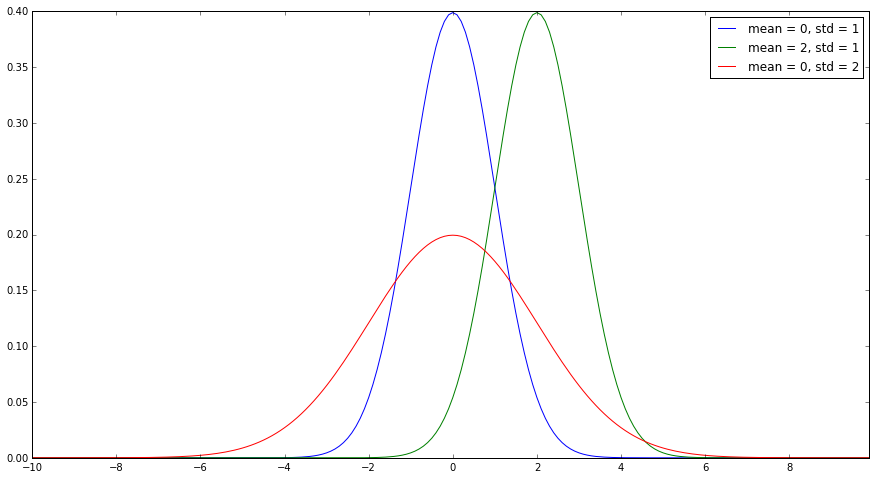
\includegraphics[scale=0.4]{../pictures/diagrams/normal-dist-example.png}\\
                        \caption{Dichtefunktionen von Normalverteilungen}\label{fig:norm-dist-pdf}
                    \end{center}
            \end{figure}

            \noindent
            Die Abbildung (\ref{fig:norm-dist-pdf}) zeigt beispielhafte Ausprägungen der Dichtefunktion, an denen man erkennen kann, dass die Standardabweichung für die Amplitute und der Durchschnitt für die Phase verantwortlich ist. Um die Wahrscheinlichkeit zu berechnen, dass eine zufällige Variable $\mathcal{X}$  mit den Grenzen $a \leq \mathcal{X} \leq b$ eintritt ist:

            \begin{figure}[H]
                \begin{mdframed}
                    \hspace*{40mm} \Resize{6cm}{$P(a \leq \mathcal{X} \leq b) = \int_a^{b} \; \mathcal{N} (\mu, \sigma^2)$}
                \end{mdframed}
                \caption{Wahrscheinlichkeit der Ausprägung $a \leq \mathcal{X} \leq b$}
            \end{figure}

            \noindent
            Diese Formel lässt sich an dem Beispiel von Regenfall pro Quadratmeter veranschaulichen:

            \begin{figure}[H]

                    \begin{center}
                        \hspace{-1cm}
                        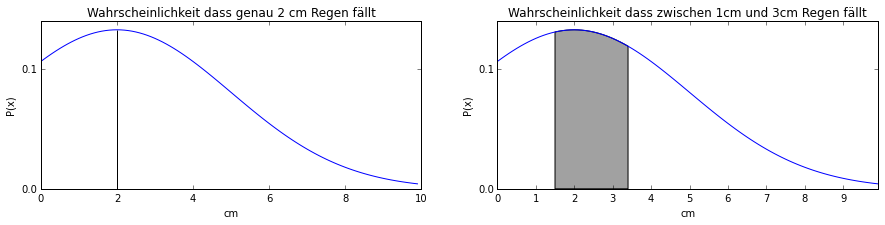
\includegraphics[scale=0.5]{../pictures/diagrams/rainfall-pdf.png}\\
%                        \caption{Kodierung der Eigenschaften durch Normalverteilungen}\label{fig:norm-dist-encoding}
                    \end{center}
            \end{figure}
            \noindent
            Die Wahrscheinlichkeit dass pro Quadratmeter \textit{genau} $2cm$ Regenwasser fällt ist extrem gering, weil nicht ein Yoctometer ($10^{-24})$ mehr oder weniger fallen darf. Wenn wir diese zufällige Ausprägung jedoch als Grenzen definieren, dann steigt die Wahrscheinlichkeit. Die Wahrscheinlichkeit dass zwischen $1cm$ und $3cm$ Regenwasser fällt ist eine viel wertvollere Aussage und ist als Integral zwischen den Grenzen der Dichtefunktion definiert.\\

            \subsubsection*{Kodierung durch Normalverteilungen}

            \begin{figure}[H]
                    \begin{center}
                        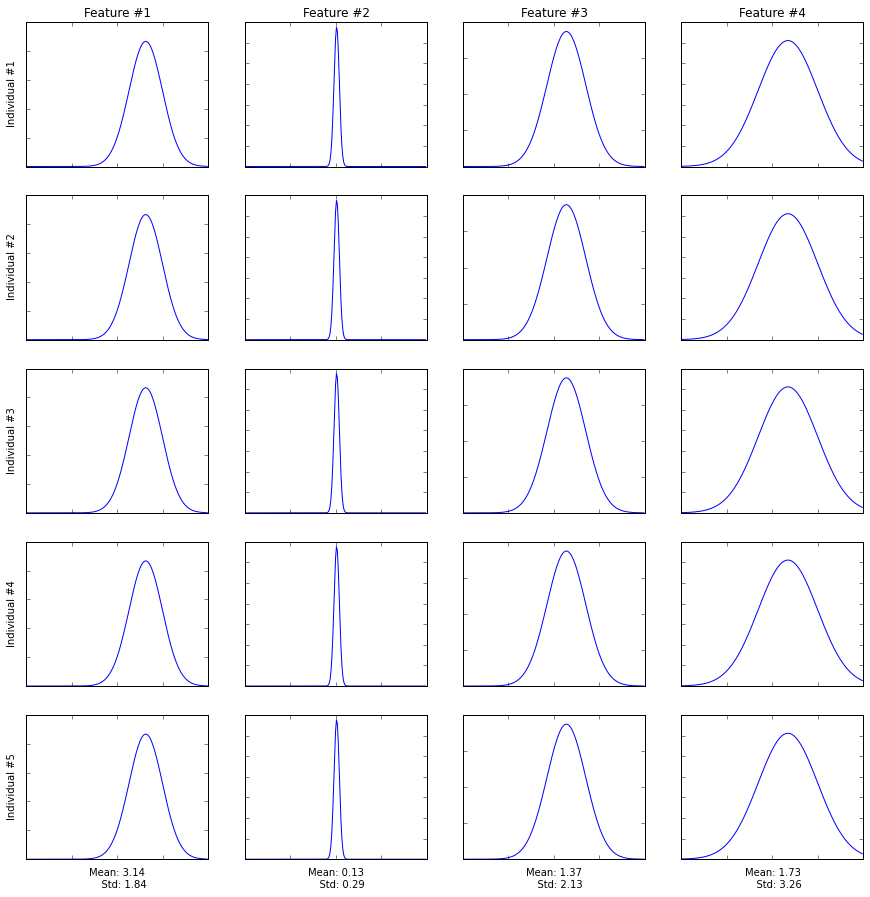
\includegraphics[scale=0.49]{../pictures/diagrams/cross-entropy-visualization-ga.png}\\
                        \caption{Kodierung der Eigenschaften durch Normalverteilungen}\label{fig:norm-dist-encoding}
                    \end{center}
            \end{figure}

            Stellen wir nun die Kodierung der Eigenschaften von jedem Individuum als Normalverteilung dar. Das bedeutet wir haben für jede Eigenschaft, zum Beispiel \textit{Hornlänge}, einen Durchschnitt und eine Standartabweichung. Die Abbilung (\ref{fig:norm-dist-encoding}) zeigt dies beispielhaft für fünf Individuen mit jeweils 4 Eigenschaften dar.\\[3mm]
            \noindent
            Wenn wir Individuen erstellen wollen, müssen wir aus jeder Normalverteilung eine Stichprobe nehmen. Die Kreuzung und Mutation fällt aus, dafür aktualisieren wir nach jeder Simulation alle Verteilungen aus den Durchschnitten und Standartabweichungen der besten Individuen.
